\chapter{Methodology}
\label{chap:methodology}

\section{Data Preparation and Splitting Strategy}

In this section the preprocessing steps and splitting strategy are introduced. In EEG classification tasks it is important to describe the steps of data preparation for both reproducibility and result interpretability. In this study the preprocessing pipeline is implemented with the goal of accurately simulating clinical practices.

\subsection{Data Preprocessing}

Before data analysis, model training, and experimentation, the raw data undergoes multiple preprocessing steps. 

\begin{description}

\item[\textbf{Removal of Constant Signal Edges:}] Some recordings contain segments where all signals are flat. These segments typically occur at the start or end of sessions and are easy to detect. During this step, all identified constant segments are removed, while the trimmed time points are recorded and the annotations are adjusted accordingly.

\item[\textbf{Temporal filtering and line-noise removal:}] Filtering changes the signal by mathematically removing unwanted parts that are in specific frequency ranges, as they are usually noise or drift rather than brain activity. A high-pass filter is applied to remove very slow changes in the signal, often caused by electrode drift due to sweat, skin potentials, or movement. A low-pass filter is also applied to remove very fast components, originating from electrical noise and muscle activity. Recordings contain a special hum-like noise from the power grid. A notch filter removes the narrow frequency band around the detected line-noise frequency, without removing the rest of the EEG spectrum.

\item[\textbf{Sampling rate validation and resampling:}] This is a simple frequency standardisation step, in which the original sampling rate of each file is checked, and if it differs from the default 250 Hz, the signal is resampled to the target rate.

\item[\textbf{Montage construction:}] The electrode signals contained in the raw EEG files are used to construct a standard set of channels, called a montage. In this specific pipeline, an average reference montage was constructed by calculating the difference between each electrode and the average of all electrodes.

\[
\tilde{x}_i(t) = x_i(t) - \frac{1}{N} \sum_{j=1}^{N} x_j(t)
\]

$x_i(t)$: electrode $i$ signal; $N$: number of electrodes; $\tilde{x}_i(t)$: average-referenced signal.

\item[\textbf{Amplitude scaling and clipping:}] Amplitudes of different EEG recordings may vary due to different amplifiers and hardware settings. For each recording, a scale factor was calculated from the middle 50\% of the absolute amplitude distribution, and global normalisation was performed, reducing sensitivity to outliers while standardising amplitude ranges across subjects and sessions. After scaling extreme EEG values were further suppressed by clipping signal amplitudes symmetrically to a threshold.

\item[\textbf{Composite label decomposition:}]

The original annotations of the TUAR dataset include composite labels like \texttt{eyem\_musc}, that represents recording segments where \texttt{eyem} and \texttt{musc} artifacts are both present. These classes are decomposed into overlapping base-label annotations to support multi-label learning. 

\item[\textbf{Z-score normalisation:}] The dataloader uses fixed-length, overlapping windows of a few seconds to segment the recordings, ensuring a consistent input representation for the models. For each window, per-channel z-score normalisation is applied to make sure all channels are on a similar scale providing consistency for the model. 

For a given window $x \in \mathbb{R}^{C \times T}$, where $C$ is the number of channels and $T$ is the number of time samples, the normalisation is defined as:

\[
z_{c,t} = \frac{x_{c,t} - \mu_c}{\sigma_c + \epsilon}
\]

$\mu_c$ and $\sigma_c$ are the average and standard deviation of channel $c$, and $\epsilon$ is a small constant added for stability.

This local normalisation prevents data leakage, helps stable training, and provides better numerical conditioning while preserving local signal structures.

\end{description}

 Each window is assigned all labels corresponding to artifact events that occur within its time interval. The preprocessing pipeline converts the raw EDF recordings into model-ready EDF files with standardised channel naming, consistent sampling rate, montage representation, amplitude normalisation, and time-aligned annotations.

\subsection{Dataset Splitting}

There are two problems with traditional dataset splitting techniques in case of window based EEG datapoints. The first one is data/patient leakage. By randomly assigning each datapoint to a split, many signal segments are going to end up in multiple splits due to the overlap of the constructed windows. In addition, patient-specific characteristics such as scalp geometry and individual brain rhythm patterns learned by the model will give unrealistic advantage in classifying the evaluation split, which misrepresents real expected performance of the model on new patients. To prevent this a patient-wise splitting technique is required. The second problem is the class imbalance in the dataset. By conducting a greedy splitting strategy, we would allow some classes to end up in a single split, which would make it impossible to train or evaluate on that class. Because of this, three mechanism were incorporated into the splitting mechanism:

\begin{description}

\item[\textbf{Patient-wise partitioning:}] Patient IDs are extracted and listed using the names of the EDF files. The files belonging to one particular patient are considered as one entity, which gets assigned to one particular split. As a result, all windows coming from the same patient get assigned to the same set, ensuring no leakage between splits.

\item[\textbf{Duration-weighted greedy assignment:}] For each patient a weight is calculated that represents the total recording time, sum of all EDF file durations in seconds of the corresponding patient. Patients are sorted from longest to shortest and assigned to the split that has its current total the furthest below its target duration. This greedy algorithm minimises the imbalance across splits.

\item[\textbf{Per-label balance objective:}] After the initial assignment, a local search performs pairwise patient swaps between the splits. A candidate swap is accepted if it decreases the total cost, where the cost is calculated using the combination of time balance error and label balance error. Time balance error is the relative squared deviation of total split duration from the target, while the label balance error is the sum, over all artifact classes, of the relative squared deviations between the annotated union duration of that class in each split and the desired class distribution across the splits. 
\newline.

\[
C = \sum_{s \in S} \left(\frac{T_s - T_s^{*}}{T_s^{*}}\right)^2
+ \alpha \sum_{l \in L} \sum_{s \in S} \left(\frac{D_{l,s} - D_{l,s}^{*}}{D_{l,s}^{*}}\right)^2
\]
\newline.

$S$ denotes the set of splits and $L$ the set of artifact labels. $T_s$ is the total recording duration of split $s$, with target duration $T_s^{*}$. $D_{l,s}$ is the annotated union duration of label $l$ in split $s$, and $D_{l,s}^{*}$ is its desired duration according to the target class distribution. The parameter $\alpha$ controls the relative importance of label balance.

This procedure iteratively improves the assignment, resulting in splits that are balanced in both total duration and artifact class representation.

\end{description}

The statistics of these optimised splits are presented in Table~\ref{tab:dataset_splits}.

\begin{table}[h]
\centering
\begin{tabular*}{\textwidth}{@{\extracolsep{\fill}}lcccc}
\toprule
\textbf{Split} & \textbf{Patients} & \textbf{Files} & \textbf{Total time} & \textbf{\% of total} \\
\midrule
Train & 182 & 235 & 75h 21m & 81.718\% \\
Dev   & 10  & 25  & 8h 27m  & 9.175\% \\
Test  & 9   & 30  & 08h 23m & 9.107\% \\
\midrule
Total & 201 & 290 & $\sim$92h & 100\% \\
\bottomrule
\end{tabular*}
\caption{Summary of dataset splits.}
\label{tab:dataset_splits}
\end{table}

\newpage

\section{Proposed  Latent Diffusion-Based Augmentation Method}

The proposed method is a latent diffusion-based synthetic data generation pipeline with similar core idea to the WGAN-GP. In the pipeline, a latent diffusion model (LDM) \cite{rombach2022} is trained to generate statistically similar datapoints to the real EEG windows from the TUAR dataset. 

For each artifact class, a separate model is used. This approach allows the models to specialise in the characteristics of a single artifact, rather than forcing a single model to learn conditional generation. The tradeoff is increased training time, memory usage, and required computational power in return for more realistic and accurate synthetic samples. During training, all datapoints corresponding to the given class are used, including the ones with multiple labels assigned. It is often considered better than using windows containing a single artifact because it avoids discarding many training samples and helps the model learn a more realistic and diverse representation of the data distribution.

In the LDM, a variational autoencoder (VAE) is combined with a denoising diffusion probabilistic model (DDPM), where first the compressed latent representation of EEG windows is learned by the VAE and then the diffusion model is trained to generate samples in this latent space. This low dimensional latent space allows the DDPM to use fewer denoising steps and maintain a lighter architecture, resulting in more efficient training and sampling. The diffusion model is trained to transform a sampled noise drawn from a gaussian distribution into a structured latent representation that reflects the learned data distribution. To achieve this, a denoising process over multiple timesteps is applied, where the model predicts and subtracts the noise component present in a given sample. Through this procedure, the model learns to reverse the forward diffusion process and generate coherent latent representations that can be decoded by the VAE into realistic EEG windows.

\subsection{Variational Autoencoder}

\subsubsection{Encoder}


First the encoder compresses the input EEG window $x \in \mathbb{R}^{B \times C \times T}$ into a low dimensional latent representation $h_\textbf{enc}  \in \mathbb{R}^{B \times C_\text{enc} \times T_\text{enc}}$ using a series of blocks each containing a 1D convolution layer with stride 2, group normalisation, and a SiLU activation function. 

\[
x \xrightarrow{\;\text{Conv + Norm + SiLU}\;} \ldots \xrightarrow{\;\text{Conv + Norm + SiLU}\;} h_\textbf{enc} 
\]

Then 1$\times$1 convolution is applied to $h$, and the tensor is split along the channel dimension to produce a Gaussian distribution for each latent variable.

\[
h_\textbf{enc}  \xrightarrow{\;\text{Conv + Split}\;} (\mu, \log \sigma^2)
\]

Using Gaussian distributions in the latent space enables stochastic sampling, allowing the model to generate synthetic EEG signal representation. 

At this point the reparameterisation trick is applied to enable differentiability. Instead of directly sampling from the distribution $\mathcal{N}(\mu, \sigma^2)$ the latent variable is redefined as: 

\[
z = \mu + \sigma \cdot \epsilon, \quad \epsilon \sim \mathcal{N}(0, I), \quad z \in \mathbb{R}^{B \times C_z \times T_z}
\]

where $\sigma = \exp\left(\frac{1}{2} \log \sigma^2 \right)$. This reformulation allows gradients to propagate through the sampling process during training.

\subsubsection{Decoder}

In the decoder the sampled latent representation $z$ is projected into a larger feature space by a 1$\times$1 convolution, where only the number of channels is modified, leaving the temporal length unchanged. 

\[
z  \xrightarrow{\;\text{Conv}\;} h_0, \qquad h_0 \in \mathbb{R}^{B \times C_d \times T_z}
\]

The decoder then applies a sequence of reconstruction blocks, where the input is upsampled with scale factor 2, followed by a convolution, group normalisation, and a SiLU activation function. 

\[
h_0 \xrightarrow{\;\text{Upsample + Conv + Norm + SiLU}\;} \ldots \xrightarrow{\;\text{Upsample + Conv + Norm + SiLU}\;} h_\textbf{dec} 
\]

After the reconstruction blocks, a finale convolution layer maps the decoder feature representation back into the original EEG signal space.

\[
h_{\text{dec}} \xrightarrow{\;\text{Conv}\;} \hat{x}, \qquad \hat{x} \in \mathbb{R}^{B \times C \times T}
\]

This decoding process enables the reconstruction of EEG signals from compact latent representations, while preserving their temporal structure.

\subsubsection{Loss Function}

During training, the VAE has two main objectives: accurate reconstruction of the EEG signal and to regularise the latent space to follow a Gaussian distribution. To achieve this, the following loss function is used: 

\[
\mathcal{L}_{\text{VAE}} = \mathcal{L}_{\text{recon}} + \lambda_{\text{KL}} \mathcal{L}_{\text{KL}}
\]

$\mathcal{L}_{\text{recon}}$ can be either L1 or MSE:

\[
\begin{aligned}
\text{L1:} \quad & \mathcal{L}_{\text{recon}} = \frac{1}{N} \sum_{i=1}^{N} |x_i - \hat{x}_i| \\
\text{MSE:} \quad & \mathcal{L}_{\text{recon}} = \frac{1}{N} \sum_{i=1}^{N} (x_i - \hat{x}_i)^2
\end{aligned}
\]

The KL divergence loss $\mathcal{L}_{\text{KL}}$ enforces $\mu \approx 0$ and $\sigma^2 \approx 1$ in the following way:

\[
\mathcal{L}_{\mathrm{KL}} = -\frac{1}{2} \sum \left( 1 + \log \sigma^2 - \mu^2 - \sigma^2 \right)
\]

The weight $\lambda_{\text{KL}}$ controls the importance of the KL divergence term in the total loss. These loss components together help the model learn both reconstruction and structured latent space representation.

\subsection{Latent Diffusion}

\subsubsection{Training}

The input of the diffusion model $z$ is the latent representation of an EEG window produced by the VAE. $z$ is scaled to have its variance normalized, because diffusion models assume inputs with approximately unit variance. 

\[
z \xrightarrow{\;\text{Scaling}\;} \tilde{z}
\]

After the scaling, a diffusion timestep $t$ is uniformly sampled from the set $\{0, \dots, T-1\}$ and Gaussian noise $\epsilon$ is generated.

\[
t \sim \mathcal{U}(0, T-1), \qquad \epsilon \sim \mathcal{N}(0, I)
\]

Using the sampled timestep and noise, along with the precomputed cumulative product of the diffusion coefficients $\bar{\alpha}_t$, the forward diffusion process corrupts the latent representation. 

\[
z_t = \sqrt{\bar{\alpha}_t}\, \tilde z + \sqrt{1 - \bar{\alpha}_t}\, \epsilon
\]

For a small $t$ value, the signal-to-noise ratio is high, but as $t$ increases, the ratio gradually decreases. 

The returned noisy tensor $z_t$ and the determined timestep scalar $t$ are passed to the denoising network. A higher dimensional vector representation of $t$ is computed using sinusoidal positional encoding. The sinusoidal embedding is passed through an MLP, consisting of two linear layers and an SiLU activation function. 

\[
t \xrightarrow{\;\text{Sinusoidal embedding}\;} \gamma(t) \xrightarrow{\;\text{MLP}\;} e_t
\]

The noisy latent tensor and the time embedding vector are given to a 1D U-Net. This denoising network consists of a downsampling path with residual blocks conditioned on the timestep, a bottleneck, and a symmetric upsampling path with skip connections. The output of the U-Net is the predicted noise component $\epsilon_\theta(z_t, e_t)$ of the input $z_t$.

\[
(z_t, e_t) \xrightarrow{\text{U-Net}} \epsilon_\theta(z_t, e_t)
\]

The goal of the training is to minimise the mean squared error between the predicted and true noise.

\[
\mathcal{L}_{\text{diff}} = \mathbb{E} \left[ \left\| \epsilon_\theta(z_t, e_t) - \epsilon \right\|^2 \right]
\]

During diffusion training, the parameters of the U-Net and the sinusoidal embedding MLP are changed, while the weights of the VAE remain fixed.

\subsubsection{Synthetic Data Generation}

In order to generate synthetic EEG windows, we need to sample from the latent distribution using the reverse diffusion process, and then transform it to a synthetic window through the decoder. The process starts with an initial Gaussian noise sample in the latent space: 

\[
z_T \sim \mathcal{N}(0, I), \qquad z_T \in \mathbb{R}^{B \times C_z \times T_z}
\]

where $z_T$ represents the corrupted latent sample at the final diffusion timestep $T$.

The model iteratively refines the latent representation by  predicting the noise component of the current latent tensor $z_t$, and estimating a less noisy latent representation at the previous timestep.

\[
(z_t, e_t) \xrightarrow{\text{U-Net}} \epsilon_\theta(z_t, e_t)
\]

\[
z_{t-1} = \frac{1}{\sqrt{\alpha_t}} \left( z_t - \frac{\beta_t}{\sqrt{1 - \bar{\alpha}_t}} \, \epsilon_\theta(z_t, e_t) \right) + \sigma_t \cdot \eta
\]

where $\beta_t$ and $\alpha_t$ are diffusion coefficients, $\sigma_t$ controls the noise scale, and $\eta \sim \mathcal{N}(0, I)$ is Gaussian noise.

After the last diffusion step $t = 0$, the final latent representation $z_0$ is rescaled to match the original latent distribution and passed to the VAE decoder, which reconstructs the final synthetic EEG window.

\[
z_0 \xrightarrow{\;\text{Unscaling}\;} \hat{z} \xrightarrow{\;\text{VAE Decoder}\;} \hat{x}, \qquad \hat{x} \in \mathbb{R}^{B \times C \times T}
\]

This method enables the synthesis of realistic EEG signals by first sampling in the structured latent space and then reconstructing them in the original signal domain.

\subsection{Overview}

The proposed method is to use this latent diffusion-based generative approach to produce fully synthetic data, add it to the original dataset, and measure the effect on artifact classification. First, the VAE is trained to learn the representation of EEG data in the latent space, then the diffusion model is trained in the latent space to model the distribution of the encoded representations. For each class, a separate model is trained to allow label specialisation. 

For the augmentation set used in training classification models, a new method is added that uses the trained LDMs for synthetic data generation. This approach enables the generation of diverse and realistic synthetic samples, which is expected to improve robustness and generalisation.

\begin{figure}[H]
\centering
    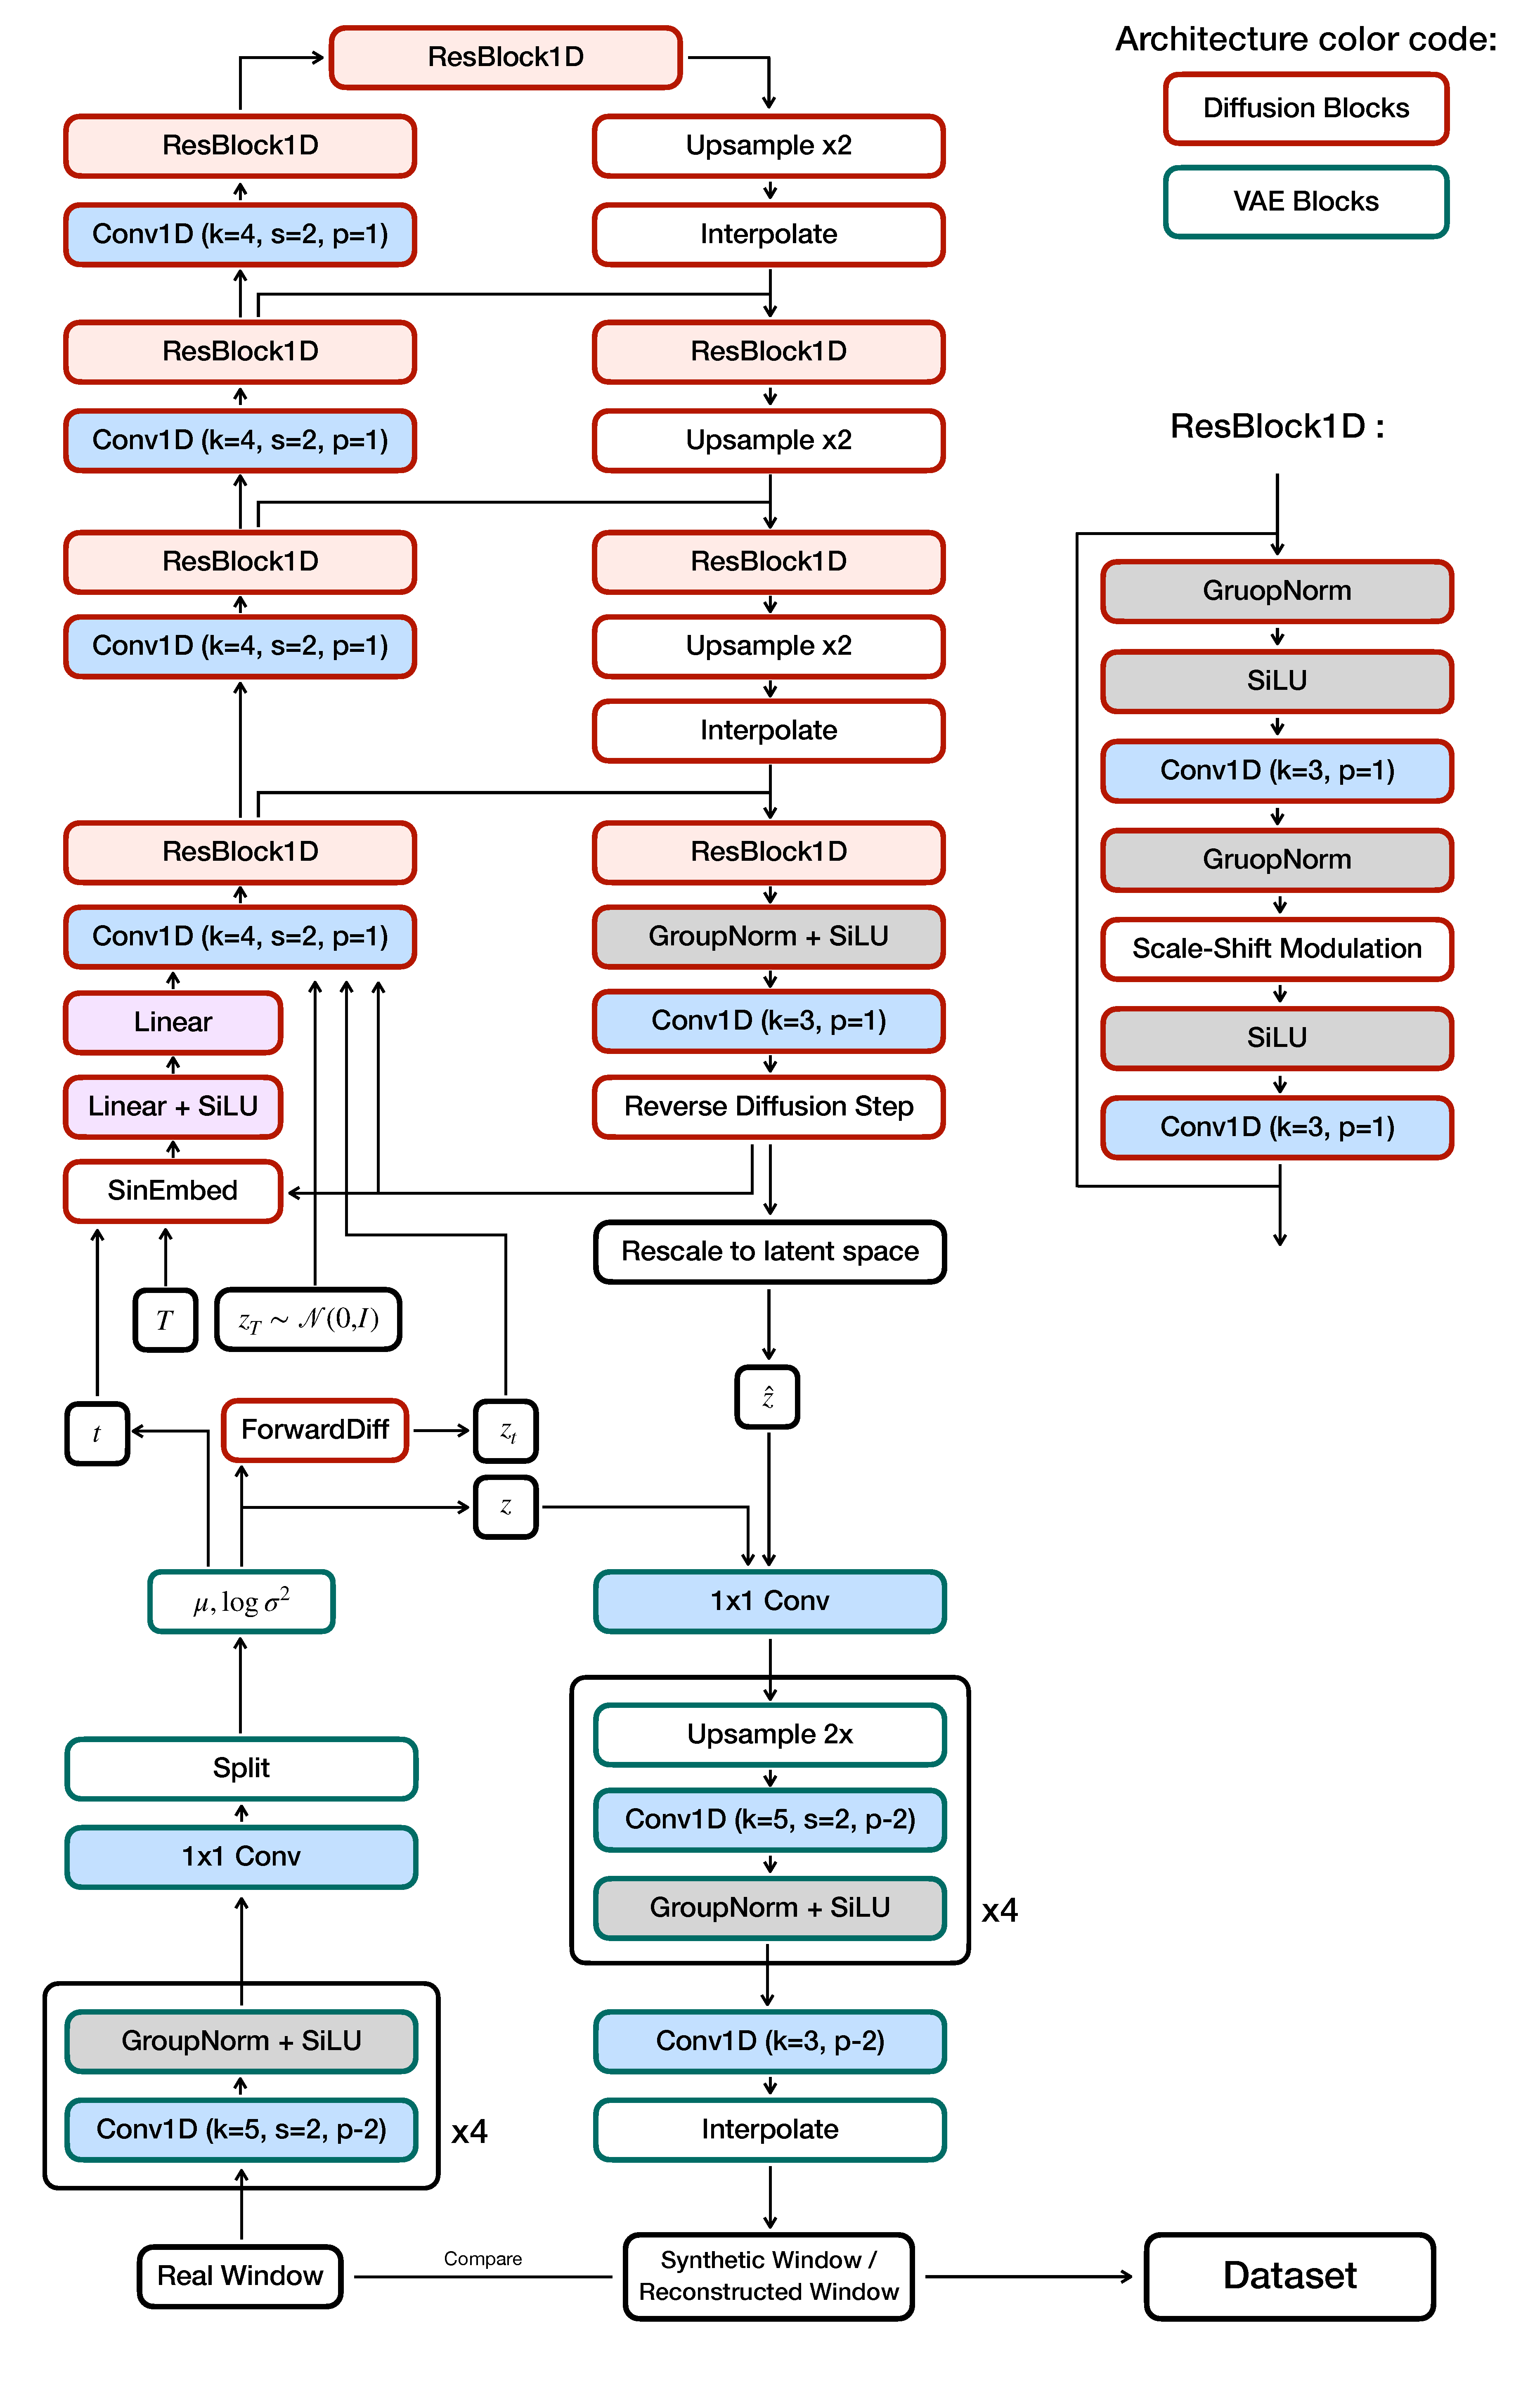
\includegraphics[width=0.9\textwidth]{images/LDM.pdf}
    \caption{Latent diffusion architecture for EEG signal generation. The VAE encodes the input $x$ into a latent $z$, which is corrupted to $z_t$ via forward diffusion. A 1D U-Net predicts and removes noise conditioned on the timestep, producing $\hat{z}$, which is decoded into the reconstructed signal $\hat{x}$.}
    \label{fig:LDM}
\end{figure}

\newpage

\section{Evaluation Metrics}

\subsection{Macro F1}

The primary metric for evaluating model performance is Macro F1-score in this study. This metric is particularly suitable for imbalanced datasets, such as TUAR, as it equally represents the contribution of minor classes and prevents dominance by majority labels. For a single class $c$, it is defined as:

\[
F1_c = \frac{2 \cdot \mathrm{Precision}_c \cdot \mathrm{Recall}_c}{\mathrm{Precision}_c + \mathrm{Recall}_c}
\]

\[
\text{Precision}_c = \frac{TP_c}{TP_c + FP_c}, \quad
\text{Recall}_c = \frac{TP_c}{TP_c + FN_c}
\]

Macro F1 is computed as the unweighted mean of the per-class F1-scores:

\[
\text{Macro F1} = \frac{1}{C} \sum_{c=1}^{C} F1_c
\]

This makes Macro F1 an accurate indicator of overall performance under class imbalance.

\subsection{Macro PR AUC}

Macro PR AUC is the secondary metric for evaluating model performance. While the F1-score evaluates using a single threshold, PR AUC measures all possible thresholds and reflects the ranking quality of the model.

For each artifact class, the PR AUC is computed separately, where each label is treated as an independent binary classification task. For class $c$, confidence scores are computed and a PR curve is constructed by varying the decision threshold.

The Macro PR AUC is defined as:

\[
\text{Macro PR AUC} = \frac{1}{C} \sum_{c=1}^{C} \text{PR AUC}_c
\]

Where $\text{PR AUC}_c$ is the area under the PR curve for class $c$.
Macro PR AUC is an informative metric in imbalanced settings, where negative samples can dominate.\\

\textbf{Additional Metrics}

Precision, recall, F1-score, and PR AUC were also monitored for performance evaluation.

\section{Experimental Design and Parameter Selection}

\subsection{Data Preparation}

\subsubsection{Window length}

Selecting the length of the EEG window is an important design decision. Shorter windows allow the model to detect short artifacts but may lack information for accurate classification. Larger window size improves the detection of longer and more complex EEG patterns but makes it harder to localise short events. The EEG recordings were sampled at 250~Hz.

To select the appropriate window length, experiments were conducted. All five classification models were trained using different window sizes. The parameter with the best metrics averaged across all models was selected. 

\begin{table}[H]
\centering
\begin{tabular}{c}
\toprule
\textbf{Evaluated window sizes (s)} \\
\midrule
1 \\
2 \\
4 \\
6 \\
\textbf{8}\\
10 \\
\bottomrule
\end{tabular}
\end{table}

The selected window size for subsequent experiments is 8~s.

\subsubsection{Stride}

The stride parameter determines the overlap between two consecutive windows. Smaller stride results in repeated samples and an increased number of windows extracted from the signal, which helps compensate imbalanced data. To determine the setting, a similar experiment was conducted as in the window size optimisation. 

\begin{table}[H]
\centering
\begin{tabular}{c}
\toprule
\textbf{Evaluated stide settings (s)} \\
\midrule
\textbf{0.5} \\
1 \\
2 \\
4 \\
\bottomrule
\end{tabular}
\end{table}

Stride of 0.5 s was selected based on the results.

\subsubsection{Sampling rate handling}

During training, a two-stage sampling strategy was used. In the first epoch, all samples were observed once, and the repeat factor of each class was calculated based on their frequencies. For the remaining epochs, the selection probabilities increased in proportion to the repeat factor of the corresponding class. The repeat factor for class $c$:

\[
r_c = \sqrt{\frac{1}{f_c}}
\]

where $f_c$ is the frequency of the given class.

Using this sampling method, the model is exposed more frequently to rare classes, which helps avoid class dominance.

\subsection{Model and Training Configuration}

\subsubsection{Batch size and learning rate}

To ensure a controlled experimental setup and isolate the effect of augmentation methods, the same batch size and learning rate were used for all classification models. These were selected by conducting multiple experiments on all models with different hyperparameter settings. The metrics were averaged across models and the parameters were selected based on the results.

\begin{table}[H]
\centering

\begin{minipage}{0.45\textwidth}
\centering
\begin{tabular}{c}
\toprule
\textbf{Evaluated batch size} \\
\midrule
32 \\
\textbf{64} \\
128 \\
256 \\
\bottomrule
\end{tabular}
\end{minipage}
\hfill
\begin{minipage}{0.45\textwidth}
\centering
\begin{tabular}{c}
\toprule
\textbf{Evaluated learning rate} \\
\midrule
$1 \times 10^{-3}$ \\
$3 \times 10^{-4}$ \\
$\mathbf{1 \times 10^{-4}}$ \\
$5 \times 10^{-5}$ \\
$1 \times 10^{-5}$ \\
\bottomrule
\end{tabular}
\end{minipage}

\end{table}

Selected parameters: batch size = 64, learning rate: $1 \times 10^{-4}$


\subsubsection{Number of epochs}

In order to determine the length of the training, an additional experiment was conducted in which all models were trained for an extended 200 epochs and the peak performance of each model was monitored. The top metrics were achieved before 40 epochs for each model. 

Based on these results, 100 epochs were selected as the final training parameter.

\subsubsection{Optimizer}

The AdamW optimizer was used for the conducted experiments in this thesis. The usage of adaptive learning rates and decoupled weight decay makes it ideal for training deep neural networks where regularisation and stable convergence are important. 

\subsubsection{Loss Function}

To handle class imbalance, Asymmetric Loss (ASL) was used as the main loss function. Let $z$ denote the predicted logit, $p$ the predicted probability, and $y \in \{0,1\}$ the target label. The loss is defined as

\[
\mathcal{L}_{\text{ASL}} = - \left[ y \log(p) + (1 - y)\log(\tilde{p}^{-}) \right] (1 - p_t)^\gamma,
\]

where $\tilde{p}^{-} = \min(1 - p + c, 1)$ is the clipped negative probability, and $p_t$ is defined as $p_t = p$ if $y = 1$, and $p_t = 1 - p$ otherwise.

Different focusing parameters are applied to positive and negative samples, making the loss asymmetric. This reduces the influence of easy negative examples and improves learning for rare classes. In this work, $\gamma_{+} = 1.0$, $\gamma_{-} = 2.0$, and $c = 0.05$ were used.

\subsection{Augmentation Settings}

\subsubsection{Non-generative augmentation parameters}

The selected parameters follow commonly used practices in EEG signal processing. These augmentation settings introduce controlled perturbations which help improve model generalisation and preserve the characteristics of the signal.

\begin{table}[H]
\centering
\label{tab:augmentation_defaults}

\begin{tabularx}{\textwidth}{l X l}
\toprule
\textbf{Augmentation} & \textbf{Parameters} & \textbf{Values} \\
\midrule
Gaussian noise           & Probability, SNR                    & 0.5, 20 dB \\
Pink noise        & Probability, SNR                    & 0.5, 20 dB \\
Temporal augmentations & Crop fraction, shift fraction       & 0.9, 0.05 \\
Segment recombination & Probability, number of segments     & 0.5, 8 \\
Channel dropout       & Probability, dropped channel fraction & 0.5, 0.1 \\
Mixup-style blending  & Probability, signal/noise ratio     & 0.5, 0.9 / 0.1 \\
\bottomrule
\end{tabularx}
\end{table}

\newpage

\subsubsection{Generative augmentation parameters}

A series of experimental trainings have been conducted in order to optimize  the hyperparameters of the generative augmentation techniques. Both the WGAN-GP and the LDM required different epoch settings for major and minor classes due to the different number of datapoints corresponding to the given label.The selected parameters are shown in the table below.

\begin{table}[H]
\centering
\begin{tabular*}{\textwidth}{@{\extracolsep{\fill}}lccc}
\toprule
\textbf{Model} & \textbf{WGAN-GP} & \textbf{VAE} & \textbf{LDM} \\
\midrule
Batch size     & 32     & 32     & 32 \\
Learning rate  & $2\times10^{-4}$ & $1\times10^{-3}$ & $2\times10^{-4}$ \\
Epoch-major    & 50     & 50     & 150 \\
Epoch-minor    & 500    & 200    & 2000 \\
Optimizer      & Adam   & Adam   & Adam \\
\bottomrule
\end{tabular*}
\end{table}

After the hyperparameter optimisation both models were trained on each class and saved for later integration into the augmentation pipeline.

\subsection{Experiments and Notation}

Two comprehensive experiments were conducted. In the first, each model–augmentation pair was trained multiple times and the average performance was measured for all pairs. The purpose of this experiment was to measure how much performance gain can be achieved using the diffusion-based method compared to baseline augmentations. By using multiple EEG classification models and conducting several trainings for each model–augmentation pair we can get wider picture of the potential of the proposed method.

The second experiment compared two existing augmentation pipelines and their combinations with two generative augmentation methods. Because augmentations are rarely used alone, it is important to test the proposed method by combining it with other techniques. The result of this experiment demonstrates the true potential of using latent diffusion-based augmentation for enhancing classification performance.

Table \ref{tab:augmentation_abbreviations} shows the set of augmentations used in the experiments and their notations for later analysis. The classification models are described in Chapter \ref{chap:background}.

\begin{table}[H]
\centering
\footnotesize
\setlength{\tabcolsep}{0pt}
\renewcommand{\arraystretch}{1.08}

\begin{tabular}{l@{\hspace{6em}}l}
\toprule
\textbf{Abbreviation} & \textbf{Method} \\
\midrule
BASE & No augmentation \\
GAUS & Gaussian noise \\
PINK & Pink noise \\
TEMP & Temporal augmentations \\
SEGR & Segment recombination \\
CHDO & Channel dropout \\
MIXU & Mixup-style blending  \\
WGAN & WGAN-GP-based generation \\
LDIF & Latent diffusion-based augmentation \\
\midrule
\multirow{2}{*}{CAP} & Composite Augmentation Pipeline \\
                     & \hspace{1.5em}PINK, TEMP, CHDO, MIXU \\
\addlinespace[3pt]
\multirow{2}{*}{CPP} & Signal Perturbation Pipeline \\
                     & \hspace{1.5em}GAUS, TEMP, SEGR \\
\bottomrule
\end{tabular}

\caption{Summary of the abbreviations used in the Results section for augmentation methods and composite pipelines.}
\label{tab:augmentation_abbreviations}
\end{table}

The Composite Augmentation Pipeline (CAP) combines pink noise injection and temporal augmentation methods with channel dropout and window blending techniques. Signal Perturbation Pipeline (CPP) replaces pink noise with Gaussian noise and combines it with segment recombination, while also including the temporal augmentation. 

Generative augmentations were combined with these pipelines with the goal of measuring their ability to further improve existing pipelines and to compare the effectiveness of the proposed latent diffusion-based method with WGAN-GP-based generation.

\subsection{Framework and Hardware}

\begin{itemize}
    \item Language and environment: Python 3.12 (conda)
    \item EEG processing framework: MNE-Python
    \item Deep learning framework: PyTorch 2.10.0
    \item CUDA: 12.8
    \item Data format: European Data Format (EDF)
\end{itemize}

All experiments were conducted on an NVIDIA GeForce RTX 2080 Ti GPU (11 GB VRAM) available on the server gpu01.cs.elte.hu provided by the Institute of Mathematics, Eötvös Loránd University.
